%!TEX root = main.tex

\section{StarCraft}
\label{sec:starcrafttheory}
\begin{figure}[h!tb]
\centering
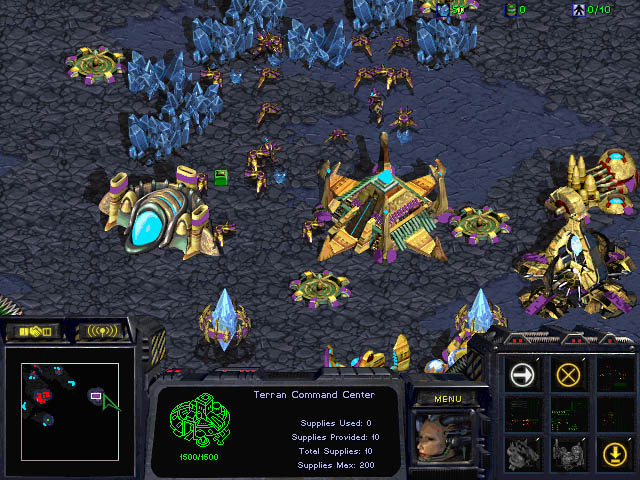
\includegraphics[scale=0.5]{graphics/scbw.jpg}
\caption{StarCraft: Brood War}
\label{fig:scbwIntro}
\end{figure}

%General introduction to the game, with emphasis on the parts that we utilize most in our project

StarCraft: Brood War is a multiplayer, real-time strategy (henceforth referred to as RTS) game, with a heavy focus on both economic strategies, as well as effective management of individual in-game units.

\subsection{Lore}
To explain some of the terms used later, it is necessary to quickly go over some of the in-game story.

\subsubsection{Setting}
The game is set far into the future, where the human race has escaped to other parts of the galaxy and started colonizing planets. Here they have discovered/been discovered by other, malevolent beings, referred to as {\em races} in the StarCraft community.
\subsubsection{Races}
There are three main races in the StarCraft universe, which are playable; the Terran (humans), Zerg and Protoss.
\paragraph{Terran} are human colonists originally from earth.
\paragraph{Zerg} is an insect-like, assimilating race. They usually rely on superior numbers.
\paragraph{Protoss} is an advanced race with powerful mental/supernatural abilities, based on {\em psionic} powers. They are both technologically and military advanced, and usually rely on few, but powerful units.

\subsection{Gameplay}
\subsubsection{Micro vs. macro}
Two well-known concepts in the RTS communities, and the StarCraft community in particular, are micro management and macro management. Macro management refers to large-scale economic and strategic decisions, while micro management refers to smaller-scale control of individual units, or groups of units.

A good control of both concepts is needed for a succesful agent.

\subsubsection{Supply}
Supply is a term for an artificial limit imposed by the game on how many units a player is allowed to make at any time. To increase the supply, a player can build a special kind of units; for the Protoss race this is {\em pylons}, for Zerg it is {\em overlords} and for Terran it is {\em supply depots}. The name stems from the terran unit needed, supply depots.

\subsubsection{Fog of war and scouting}
Fog of war is a well-known term from RTS games, which denotes un-observed parts of the environment or map. In StarCraft this is shown as shaded on screen. This leads to partial observability, and gives rise to uncertainty about the rest of the map, about what the other player is doing and what resources he has exhausted. To counteract this, it is common to {\em scout}, that is, to send out units to simply observe the other player.

\subsection{BWAPI}
To ease the development of third-party agents that play the game, an application programming interface (API) has been developed for StarCraft: Brood War, by third-party developers. They have relied on reverse engineering of the original game for developing it. It works by injecting itself into the process of the game, and hooking into various functions used in the game, as well as reading various memory areas directly.\cite{bwapi}

There has sprung up a sizeable community around this effort, and there are several tournaments where programmers can participate with their own agents.\cite{bwapi}

There are also several third-party addons and extra libraries for easing the development of agents, such as the Brood War Terrain Analyzer (BWTA), which provides easy-to-use functions for analyzing the maps for finding choke-points and suitable locations for various buildings,\cite{bwta} and the Brood War Standard Addon Library (BWSAL) which is both a generic, modular framework for BWAPI agents as well as default implementations for a large part of the modules needed for implementing such an agent.\cite{bwsal}

BWAPI only provides a C++ API, so for using it from other languages various types of bindings are needed.

There are two modes for loading agents using BWAPI; loading it directly into the StarCraft process, or using a shared-memory area to communicate state between the agent process and the StarCraft process in which the BWAPI code is running.\cite{bwapi}

\subsubsection{JNIBWAPI}
For using Java for developing an agent the most well-supported is using the JNIBWAPI project, which uses JNI to provide Java-bindings for BWAPI. It utilizes the shared-memory approach of BWAPI to avoid having to load the Java bytecode interpreter into the StarCraft memory.
